\section{Einleitung}
\label{einleitung}
Dieses Dokument wurde im Rahmen des Masterprojekts des Studiengangs Informatik an der HTWK-Leipzig erstellt. Es beinhaltet die Entwicklung und prototypische Umsetzung eines Chatbots für die Terminverwaltung des Studentenclubs \glqq Stecker\grqq .

Der Auftrag wurde von der technischen Abteilung des Clubs gestellt. Die Motivation hierfür ist eine einfache, schnelle und zentrale Verwaltung von Schichtplänen, um den Vorstand in der Organisation der Veranstaltungen zu entlasten.
Es wird ein Chatbot benötigt, welcher über die Kommunikationsplattform \glqq Slack\grqq gesteuert werden kann und auch von technisch nicht versierten Mitgliedern bedienbar ist.

Dieses Dokument wird die Anforderungen an den Chatbot präsentieren und bereits vorhandene Lösungen bewerten und gegenüberstellen. Anschließend wird ein Modell für die Verwendung eines Frameworks im Zusammenhang mit Use-Cases erstellt. Weiterhin wird ein Datenbankmodell für die Terminverwaltung entworfen, welches sich nicht nur auf die bekannten Anwendungsfälle beschränken wird. Es wird gesondert auf die praktische Realisierung und die zu beachtenden Probleme bei der Einrichtung eingegangen. Das fertige System wird anschließend Analysiert und Bewertet. Im Schlusswort werden die Autoren das entworfene System den Anforderungen gegenüberstellen und abschließend eine Aussicht für die weitere Entwicklung geben.
% kurz Abstract
% um was gehts, wer gab den auftrag, welcher hintergrund / motivation
% was ist das grobe ziel

\clearpage
\section{Anforderungen und Festlegungen}
\label{anforderungen}
\subsection{Anforderungen des Auftraggebers}
Der Auftraggeber teilt seine Anforderungen in notwendige und optionale Ziele ein, welche nachfolgend aufgelistet werden. Als notwendige Ziele für das Projekt wurden folgende festgelegt.

\begin{itemize}
	\item Chatbot ist in Slack verwendbar
	\item Datenbank, welche Veranstaltungen und Zuweisungen der Mitglieder enthält
	\item Erfassung, welche Mitglieder wie viele Dienste gemacht haben
	\item Abfragefunktion ist für Termine vorhanden
	\item zeitgesteuerte, ereignisbasierte und manuelle Erinnerungsfunktion
	\item Einschränkung der Zielgruppe bzgl. Erinnerungen möglich
	\item einfache Bedienbarkeit
	\item Erweiterbarkeit des Projekts gegeben
	\item MIT-ähnliche Lizenzen für Drittanbietersoftware und -quelltext
	\item Dokumentation der Datenbank
	\item Unabhängigkeit der relevanten Daten vom verwendeten Bot
	\item Zukunftssicherheit
\end{itemize}


Die optionalen Ziele werden nachfolgend aufgeführt.
\begin{itemize}
	\item aus iCal Termine extrahieren
	\item Dienstplan aus Doodle-ähnlicher Umfrage erstellen
	\item Nutzerberechtigungen
	\item Steuerung über E-Mail
	\item containerbasierte Lösung
	\item Caching für schnellere Abfragen
	\item Backup-Strategie
\end{itemize}

% Hier schon das Usecase-Diagramm hin? - NEIN, hier kommt nur das rein, was Ferdi gesagt hat. Alles was wir selbst erarbeitet haben kommt danach.

\subsection{Festlegungen}
% Synonyme, Beschreibungen, Abgrenzungen für die Arbeit

Eine Menge an Terminen wird mit $T$ bezeichnet, Veranstaltungen mit $V$ und Sitzungen mit $S$.

Alle im Rahmen dieser Arbeit erstellten UML-Diagramme entsprechen dem aktuellen UML-Standard, Version 2.5.1. Dieser steht unter \url{https://www.omg.org/spec/UML/2.5.1/} zur Verfügung.

Alle das System nutzenden Akteure werden im Folgenden als Nutzer bezeichnet. Mitarbeiter sind alle Mitarbeiter des Studentenclubs Stecker. Administratoren sind spezielle Nutzer mit zusätzlichen Berechtigungen.
Es bestehen folgende Abhängigkeiten: 

$Nutzer = Administrator \cup Mitarbeiter$ 
%und $Administrator \subset Nutzer$ // unnötig

\subsection{Anwendungsfalldiagramme}

% ??????????? Das klingt eher wie ein Vorwort für den Entwurf der Digaramme. ich würde hier nur Dinge rein schreiben, die sich über mehrere Kapitel erstrecken, so als "globale variablen"
% Ich würde die UML-Usecases schon gern einleiten, wirkt sonst so lieblos, sollen ja auch einen Sinn haben

Die auf den vorherigen Seiten zusammengetragenen obligatorischen Projektziele wurden zur besseren Überprüfung der Ziele in Anwendungsfälle umformuliert. Diese wurden entsprechend \autoref{usecase-auftrag} auf die Akteure \enquote{Bot} und \enquote{Auftraggeber} verteilt.

Die Auftraggeber sind hierbei Ferdinand Malcher und Robert Weisse als Angehörige des Studentenclubs \enquote{Stecker}. Der \enquote{Bot} ist eine nicht näher spezifizierte Chatbot-Technologie, die aber bewusst als Akteur eingeführt wurde, da sie selbständig Aktionen ausführen soll.

\begin{figure}[htbp]
    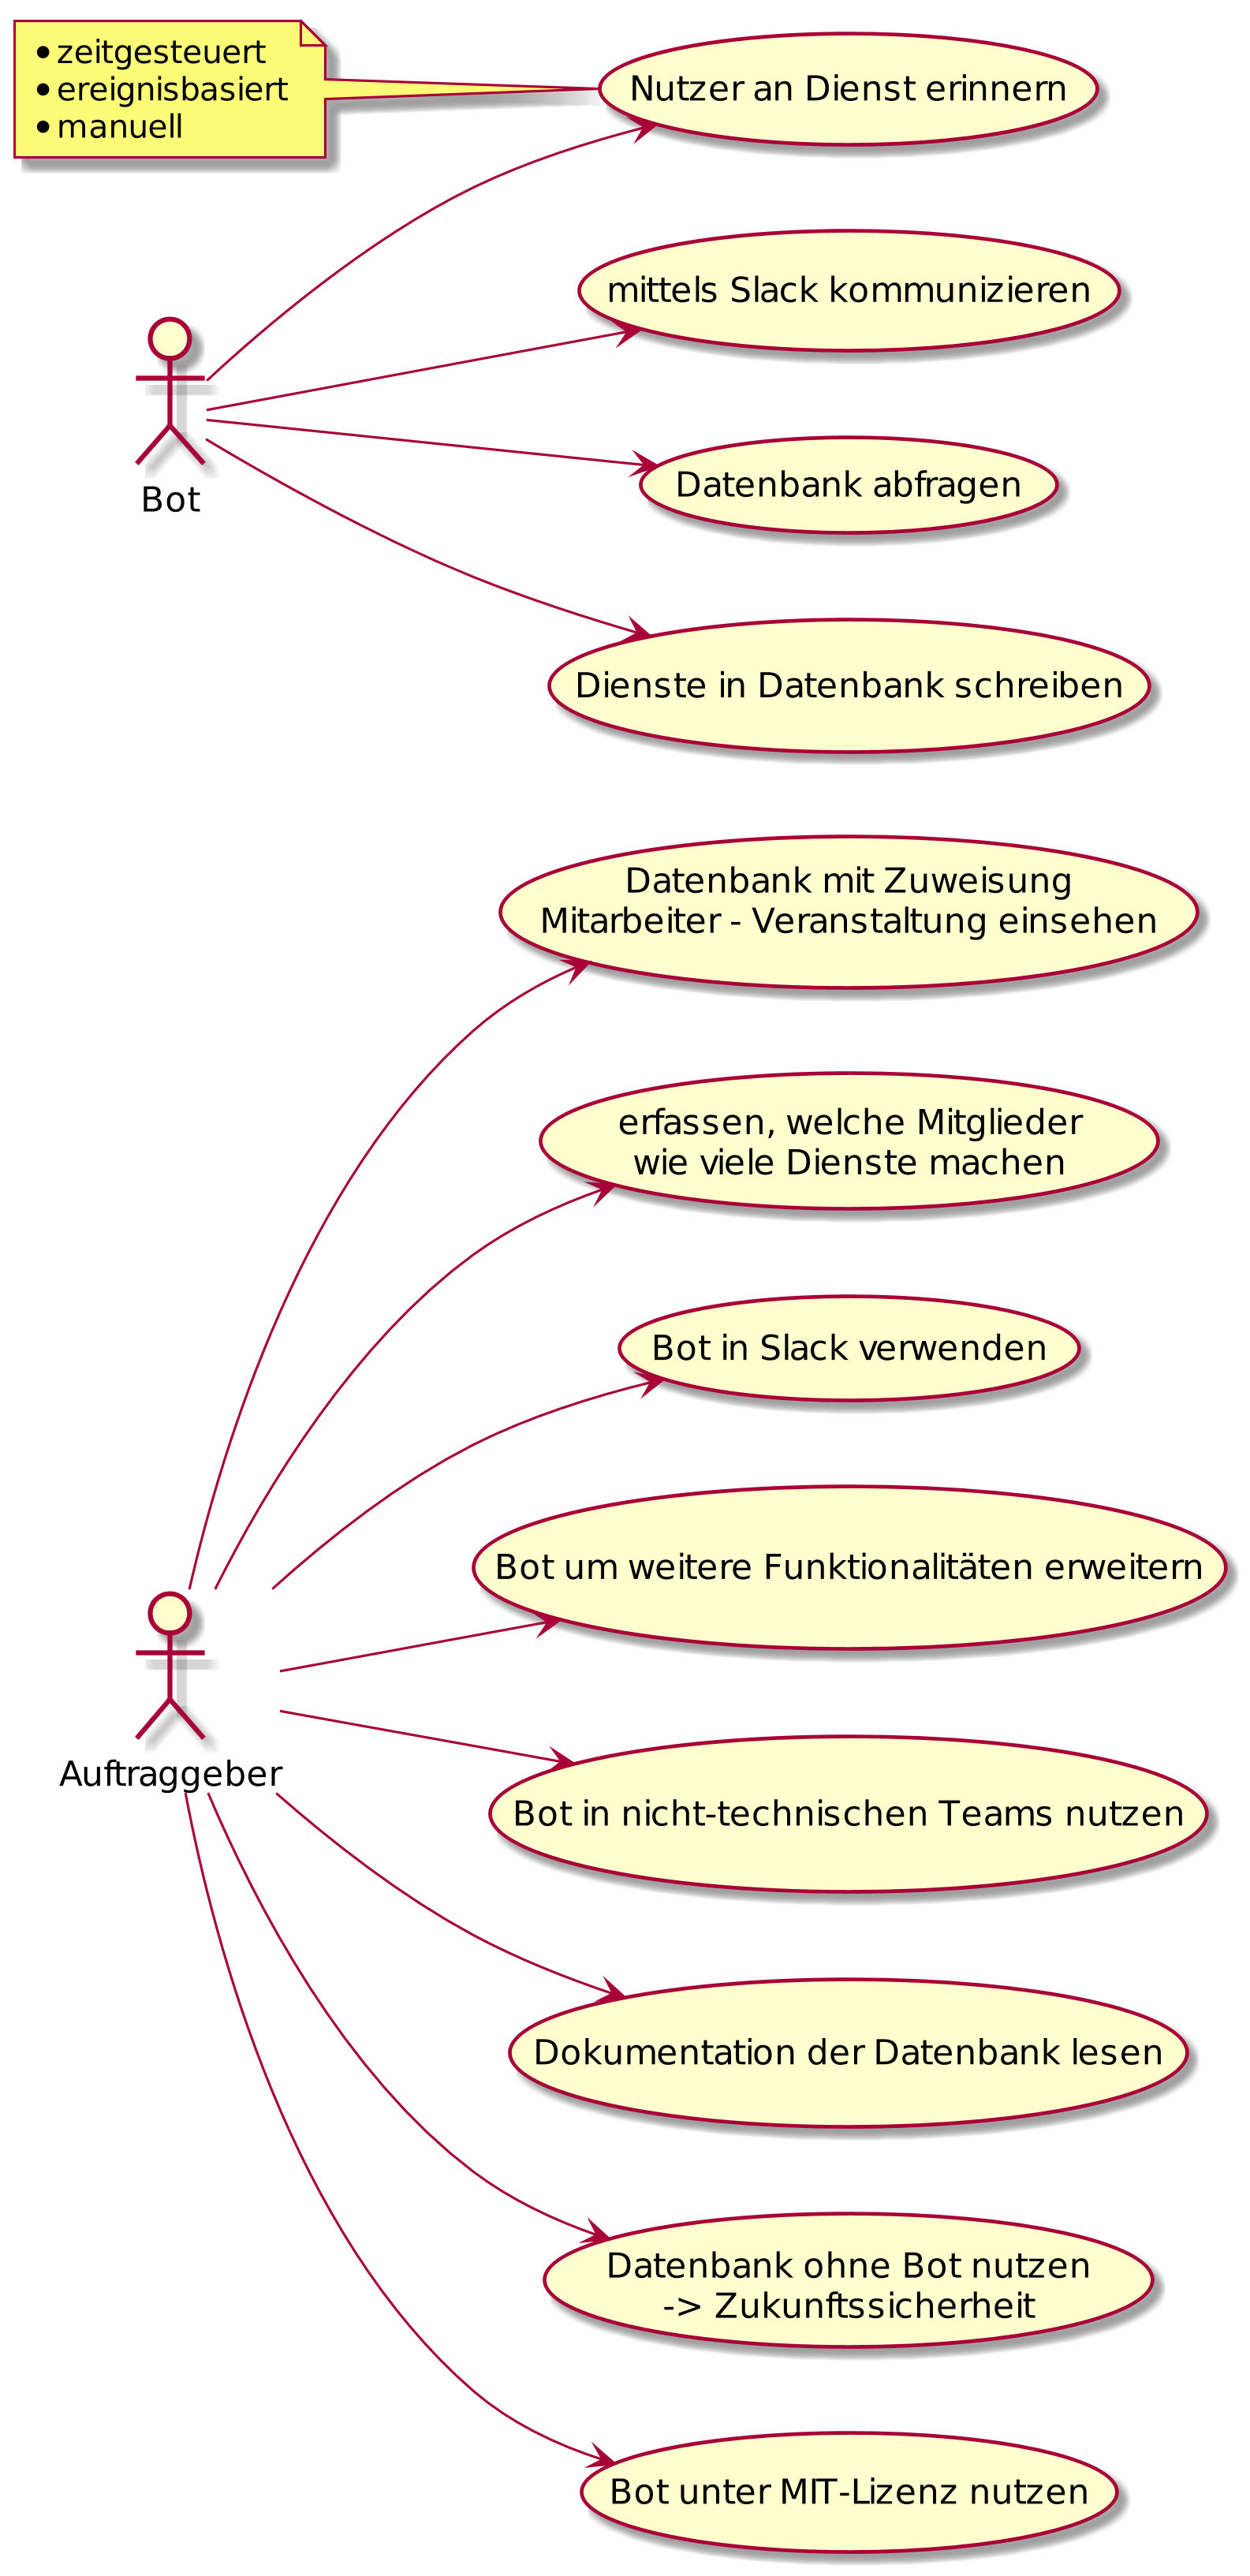
\includegraphics[width=0.7\textwidth]{../docs/uml/usecase-stakeholder.png}
    \caption{Anwendungsfalldiagramm für Auftraggeber und Bot}
    \label{usecase-auftrag}
\end{figure}


Für den zukünftigen Einsatz wurde ein weiteres Anwendungsfalldiagramm zur Unterteilung der Berechtigung der Nutzer erstellt. Gemäß Aufgabenstellung sind in \autoref{img:usecase-berechtigung} die Anwendungsfälle der Nutzer beschrieben. Die darin ebenfalls enthaltene Unterteilung der Berechtigungen dient hier nur der Vollständigkeit, da diese nicht zur initialen Aufgabenstellung gehört.
Eine weitere mögliche Betrachtung ist der unterschiedliche Grad an Fähigkeiten zwischen Administrator und Mitarbeiter. Während es einem Administrator zumutbar ist, beispielweise einen Nutzer direkt per Datenbankzugriff anzulegen, so benötigt der Mitarbeiter eine seinen Fähigkeiten angemessene Schnittstelle wie sie der Chatbot bieten soll.

\begin{figure}[htbp]
    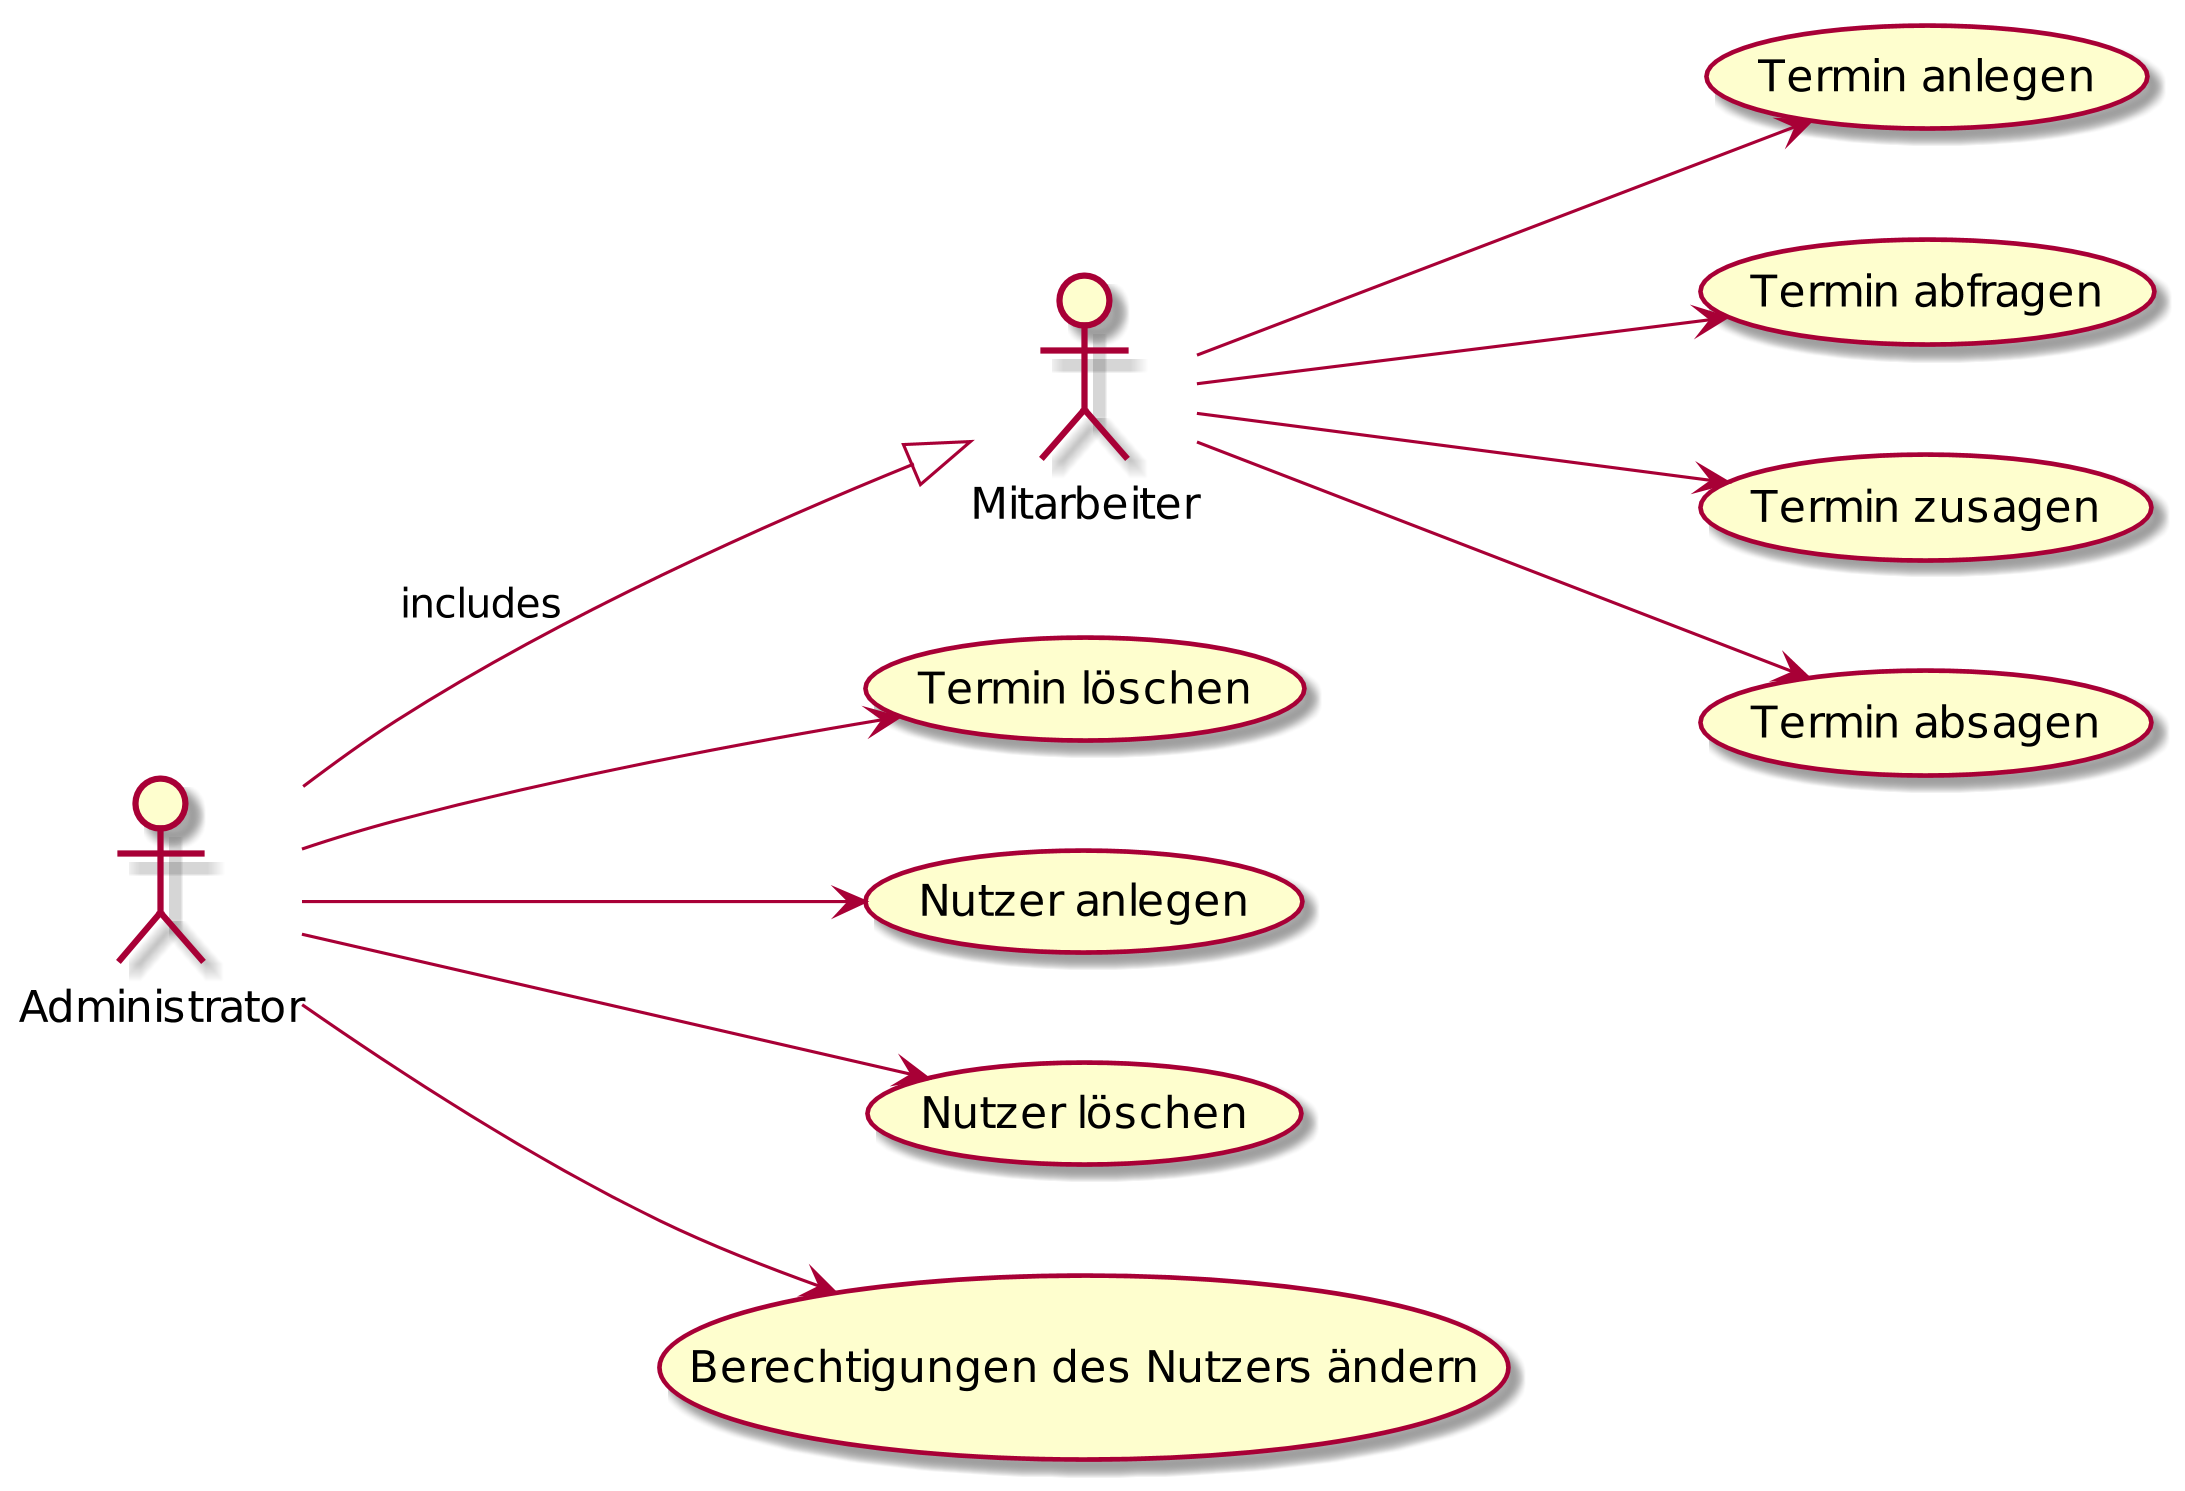
\includegraphics[width=0.9\textwidth]{../docs/uml/usecase-berechtigung.png}
    \caption{Anwendungsfalldiagramm zur Abgrenzung von Mitarbeiter und Administrator}
    \label{img:usecase-berechtigung}
\end{figure}
% Ferdi will, Ferdi verlangt, Ferdi lässt Spielraum (feine ziele)
% Festgelegte Begriffe, allgemeingültige Aussagen für das Dokument

\clearpage
\section{Auswahl eines Bot-Frameworks}
\label{botframework}

\subsection{Vergleichsparameter}
Für einen Vergleich der einzusetzenden Bot-Frameworks werden für diese im Folgenden Vergleichsparameter definiert. Dabei ist es wichtig, diese an den Anforderungen aus dem vorherigen Kapitel sowie technischen Aspekten zu orientieren.

Jeder Parameter muss folgende Kriterien erfüllen:

\begin{itemize}
    \item messbar, als Zahlen- Text- oder Wahrheitswert
    \item generisch, d.h. auf die zu vergleichenden Frameworks anwendbar
    \item nachweisbar, d.h. die Herkunft des Wertes ist nachvollziehbar
\end{itemize}

Aus \autoref{tab:botparameters} sind passende Bewertungsparameter gemäß der oben genannten Anforderungen zu entnehmen.

% evtl. booktabs statt tabularx
\begin{table}[htbp]
    \begin{tabularx}{\textwidth}{|l|X|p{6cm}|}
   \hline
   \textbf{Parameter} & \textbf{Beschreibung} & \textbf{Quelle} \\
   \hline
   Alter & Datum des ersten Commits im Master-branch & \verb+git log --reverse | head -3+\\
   \hline
   Aktivität & Commits in den Master-branch, Anz.\ Pull-Requests & GitHub Projektübersicht \\
   \hline
   Popularität & Anz.\ \enquote{Stars} und \enquote{Forks} & GitHub \\
    \hline
   Codequalität & Testabdeckung und Anz.\ Issues & GitHub, Tests vorhanden \\
   \hline
   Komplexität & Anz.\ Klassen, SLOC\footnote{Source Lines of Code}, Dateigröße \textbf{ohne Beispiele, externe Abhängigkeiten etc.} & \verb+du+, Code, \verb+git ls-files | xargs wc -l+ \\
   \hline
   Programmiersprache & primär verwendete Programmiersprache & GitHub-Seite \\
   \hline
   Integrationsgrad & Anz.\ bereits vorhandener Integrationen & Website, Dokumentation, npm \\
   \hline
   Erweiterbarkeit & Anz. der Erweiterungsmodule & Code, Dokumentation \\
   \hline
   Dokumentation & Dokumentation vorhanden ja/nein & docs-Ordner oder GitHub-Wiki \\
   \hline
   Lizenz & Art der Lizenz des Projektes & LICENSE.md im Git-Repositorium \\
   \hline
\end{tabularx}
\caption{Parameter zum Vergleich der Bot-Frameworks}
\label{tab:botparameters}
\end{table}

Die Aussagefähigkeit der in \autoref{tab:botparameters} enthaltenen Parameter ist stellenweise kritisch zu hinterfragen, da die Genauigkeit zugunsten der Generizität eingeschränkt wurde. 
Beispiele hierfür sind folgende:
\begin{itemize}
    \item Testabdeckung: je nach Auswahl und Integration der Testbibliothek kann die Testabdeckung immer 100\% betragen
\item SLOC: viele Codezeilen deuten nicht zwingend auf guten Code hin (von Kommentaren wird hier, per Definition, abgesehen)
\end{itemize}

Unter Beachtung der Einschränkungen und der Kombination aller Parameter ist eine differenzierte Gegenüberstellung durchführbar.

\subsection{Auswahl möglicher Frameworks}

Aufbauend auf den zu Beginn gestellten Anforderungen entfallen Frameworks:
\begin{itemize}
    \item deren Quelltext nicht frei verfügbar ist
    \item die eine dauerhafte Verbindung zum Hersteller benötigen
    \item die nicht kostenfrei sind
\end{itemize}

Durch diese Einschränkungen sind z.B. das von facebook entwickelte wit-Botframework (\url{https://wit.ai/}) und das von Microsoft entwickelte Bot-framework (\url{https://dev.botframework.com/}) nicht Teil weiterer Betrachtungen.
Eine weitere Gruppe von Botframeworks zeichnet sich durch eine (meist zwingende) Anbindung an eine Spracherkennung aus, die für den hier gewünschten Anwendungsfall nicht benötigt wird. Dadurch wird z.B. \url{api.ai} nicht Teil weiterer Betrachtungen sein.


Weitere Botframeworks sind unter \url{https://github.com/abdelhai/awesome-bots} aufgelistet. 
Von den dort aufgelisteten Frameworks entsprechen hier \textbf{Botkit} (\url{https://botkit.ai/}) und \textbf{Hubot} (\url{https://hubot.github.com/}) den Anforderungen.

\subsection{Vergleich der Frameworks}

\begin{table}[htbp]
    \centering
    \begin{tabularx}{\textwidth}{|l|X|X|}
        \hline
        \textbf{Parameter} & \textbf{Botkit} & \textbf{Hubot} \\
        \hline
        Alter (Stand 02.2018) & $\approx$ 2 Jahre & $\approx$ 5 Jahre \\
        \hline
        Aktivität & \makecell[l]{2078 Commits\\ 29 Pull-Requests} & \makecell[l]{2011 Commits\\ 5 Pull-Requests} \\
        \hline
        Popularität & \makecell[l]{7.813 Sterne\\ 1.714 Forks} & \makecell[l]{13.817 Sterne\\ 3.269 Forks} \\
        \hline
        Codequalität & \makecell[l]{115 Issues\\ Testabdeckung 100\%} & \makecell[l]{30 Issues\\ Testabdeckung 100\%} \\
        \hline
        Komplexität & 35259 SLOC & 7472 SLOC \\
        \hline
        Programmiersprache & TypeScript & CoffeeScript \\
        \hline
        Integrationsgrad & 12 & 62 \\
        \hline
        Erweiterbarkeit & 28 & $\approx$ 50 \\
        \hline
        Dokumentation & ja & ja \\
        \hline
        Lizenz & frei, MIT & frei, MIT \\
        \hline
    \end{tabularx}
    \caption{Vergleich von Botkit und Hubot}
    \label{tab:comparebotkithubot}
\end{table}

% Zwischenfazit: Botkit ist größer und umfangreicher, Hubot kleiner und simpler.
% Würde ich am Ende von TypeScript vs. CoffeeScript abhängig machen

Wie in \autoref{tab:comparebotkithubot} ersichtlich, bietet Hubot aufgrund der längeren Entwicklungszeit eine größere Anzahl von Nutzern und Integrationen. Des Weiteren ist Hubot auf die praktische Notwendigkeit bei GitHub zurückzuführen, die Entwicklungsprozesse an ChatOps\footnote{Ausführen von Deployment-Befehlen etc. direkt aus dem Chat-Programm, Hintergrund siehe: \url{https://www.youtube.com/watch?v=NST3u-GjjFw}} auszurichten.

Im Gegensatz dazu bietet Botkit flexiblere Einsatzmöglichkeiten und Integrationen in andere Dienste wie NLU\footnote{Natural language understanding}, Apps und Messenger. Aufgrund des relativ jungen Projektalters von zwei Jahren und der vergleichsweise höheren Anzahl an Bugtickets (\enquote{Issues}) und Codezeilen, wird die Codequalität Botkits geringer als die Hubots bewertet.

Beide Frameworks dienen dabei unterschiedlichen Zielen: während Botkit eher als Rahmenwerk für darauf aufbauende Bots anzusehen ist, ist der Bot als solches direkt bei Hubot integriert und kann modular erweitert werden. Da beide Frameworks unter MIT-Lizenz stehen und zu JavaScript kompilieren, sind diese aus lizenzrechtlicher und technischer Sicht für das Projekt \enquote{Steckerbot} geeignet.

Für den in \autoref{anforderungen} beschriebenen Einsatzzweck fällt die Entscheidung auf \textbf{Hubot}. Im Vergleich zu Botkit bewerten die Autoren Hubot als strukturell simpler und näher am Ziel der praktischen Slack-Integration ausgerichtet. Botkit erfüllt diese Anforderungen auch, hatte jedoch keine so lange Reifephase wie Hubot.

Im weiteren Verlauf dieses Dokuments werden deshalb \enquote{Hubot}, \enquote{Botframework} und \enquote{Bot} synonym verwendet.


% HuBot, BotKit
% Einschränkungen der Auswahl weil ...

\clearpage
\section{Entwurf eines Modells}
\subsection{Anforderungsanalyse mittels Use-Case-Betrachtung}
% TODO: Struktur der Überschriften ändern, diese hat nur einen 
% Unterpunkt und passt thematisch nicht

\subsubsection{Interaktion über Slack}

Es werden folgende Befehle für die Interaktion definiert.

\begin{table}[H]
\centering
\begin{tabular}{l|l}
  Befehl & Bedeutung \\
 \hline
% für vergessliche Leute
 zeige Schicht & zeigt die nächste Schicht für die aufrufende Person an \\
 zeige Schichten & zeigt alle zukünftigen Schichten für die aufrufende Person an \\
 zeige alle Schichten & zeigt einen Schichtplan an, welcher alle Mitglieder enthält \\
 
% jedes Mitglied muss pro Jahr mindestens x mal an die Bar
 zeige Anzahl Schichten & zeigt die geleisteten Schichten für dieses Jahr an \\
 zeige Anzahl alte Schichten & zeigt die geleisteten Sichten für letztes Jahr an \\
 
% zum Anzeigen der Auswahl an welchen man teilnehmen  möchte
 zeige Termine & zeigt alle kommenden Termine $t_i$ an \\
 zeige Veranstaltungen & zeigt alle zukünftigen Veranstaltungen $v_i$ an ($V \subseteq T$) \\
 zeige Sitzungen & zeigt alle zukünftigen Sitzungen $s_i$ an ($S \subseteq T$) \\
 
% für Termin eintragen
 nehme Teil an $t_i$ & trägt den aufrufenden Nutzer als Teilnehmer für $t_i$ ein \\
 nehme nicht Teil an $t_i$ & trägt den aufrufenden Nutzer für $t_i$ aus\\

 % Utilities
 hilf mir & zeigt alle verfügbaren Kommandos an \\
 Danke & bricht die aktuelle Konversation ab
 
 wann ist der nächste termin?
 trag mich ein
 
 
\end{tabular}
\caption{Befehle zur Chatbotinteraktion}
\label{tab:chatbotinteraktion}
\end{table}

Die Befehle in \autoref{tab:chatbotinteraktion} folgen einem vereinfachtem Schema natürlicher Sprache: $<Prädikat (Imperativ)> <Subjekt>$. Die Struktur der Befehle soll dabei einfach zu merken, auf menschlicher Sprache basierend und auch auf mobilen Geräten mit wenig Tipparbeit verwendbar sein. Bei einem optionalen Einsatz einer Spracherkennung sind auch komplexere Satzkonstruktionen möglich, für den hier zu erfüllenden Zweck genügt das Schema aus $<Befehl> <Objekt> <Filter>$. Wie in \cite{ZueConversationalinterfacesadvances2000} beschrieben, weicht die Art der Kommunikation von Mensch-zu-Mensch und Mensch-zu-Bot voneinander ab, worauf bei der Definition der Interaktionsbefehle geachtet wurde. Es ist nach Ansicht der Autoren wenig sinnvoll, einen Bot zu entwickeln, der durch den Zugriff auf große Datenmengen den Eindruck von Intelligenz vermittelt, die aber durch ihre Begrenzung dem Nutzer keinen Mehrwert bietet. Der hier entwickelte Bot verfügt bewusst über ein begrenztes Vokabular, so dass er nur die vom Nutzer gewünschten Informationen liefert; die Kenntnis der Befehle obliegt dem Nutzer.

Aus den in \autoref{tab:chatbotinteraktion} definierten Befehlen wurden die Aktivitätsdiagramme \autoref{img:activity-zeige} und \autoref{img:activity-teilnahme} erstellt, um die Reihenfolge der Interaktion besser zu strukturieren.

\begin{figure}[htbp]
    \centering
    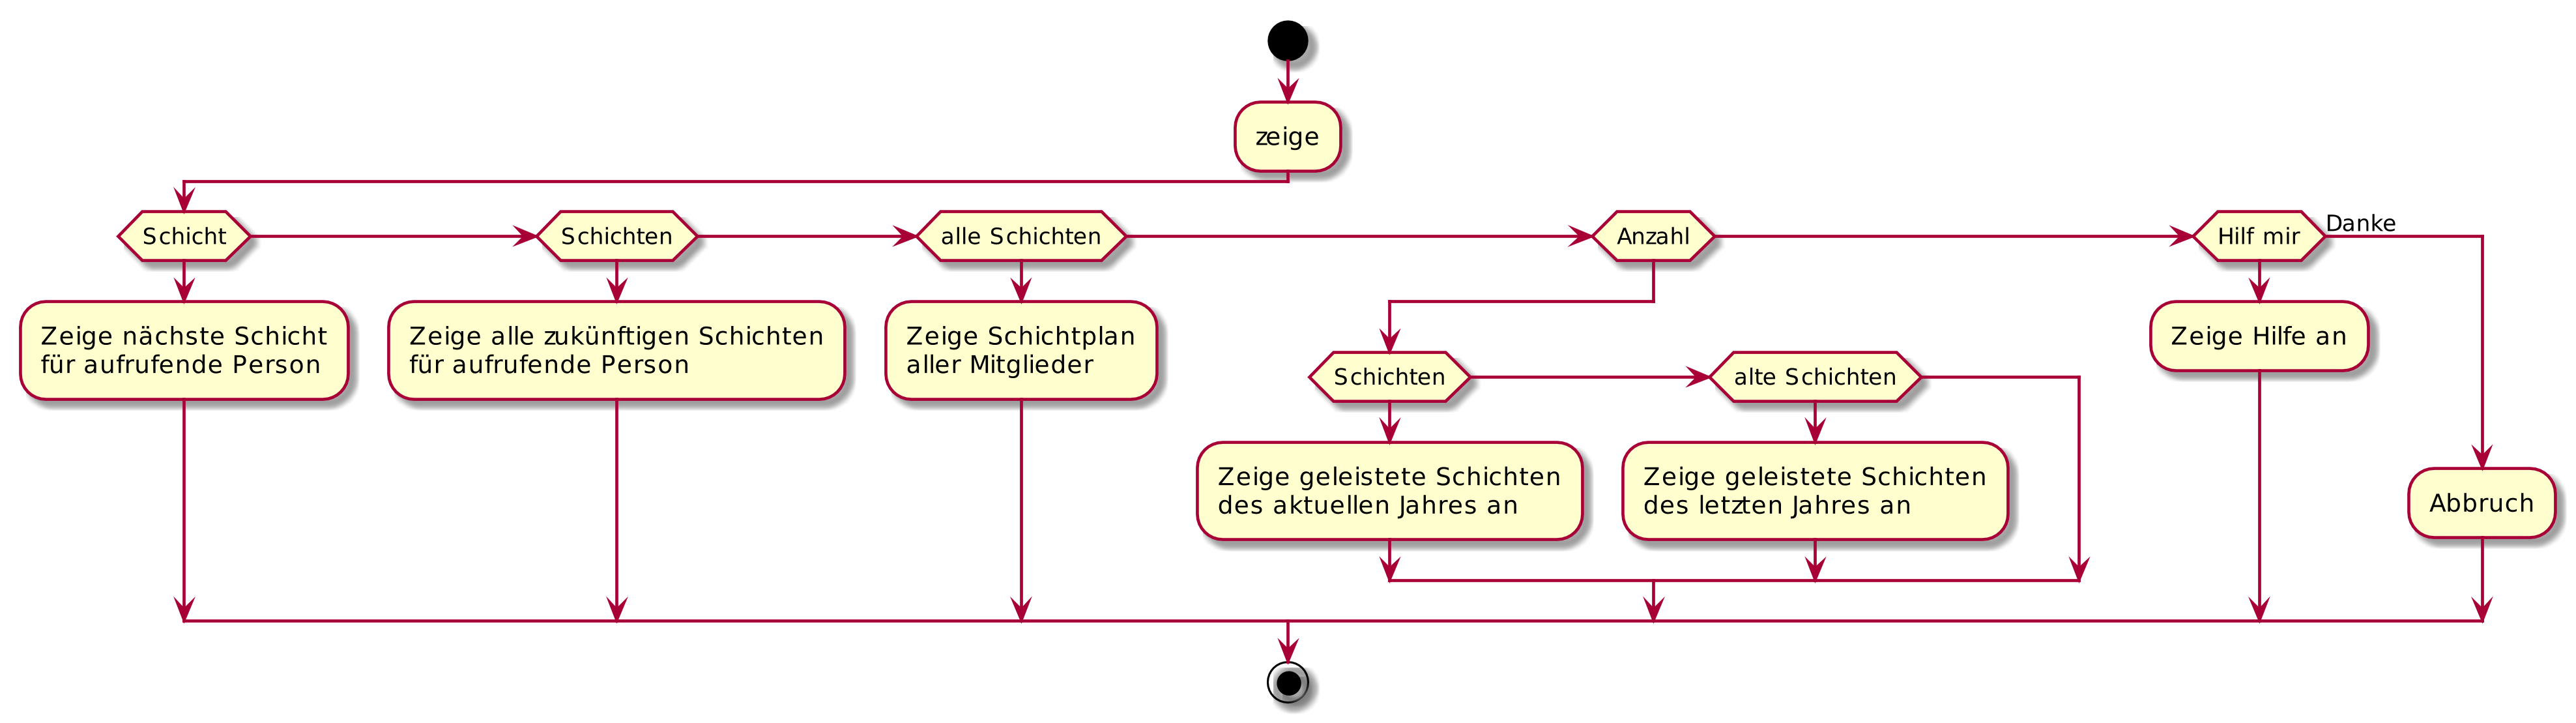
\includegraphics[width=\textwidth]{../docs/uml/activity-zeige.png}
    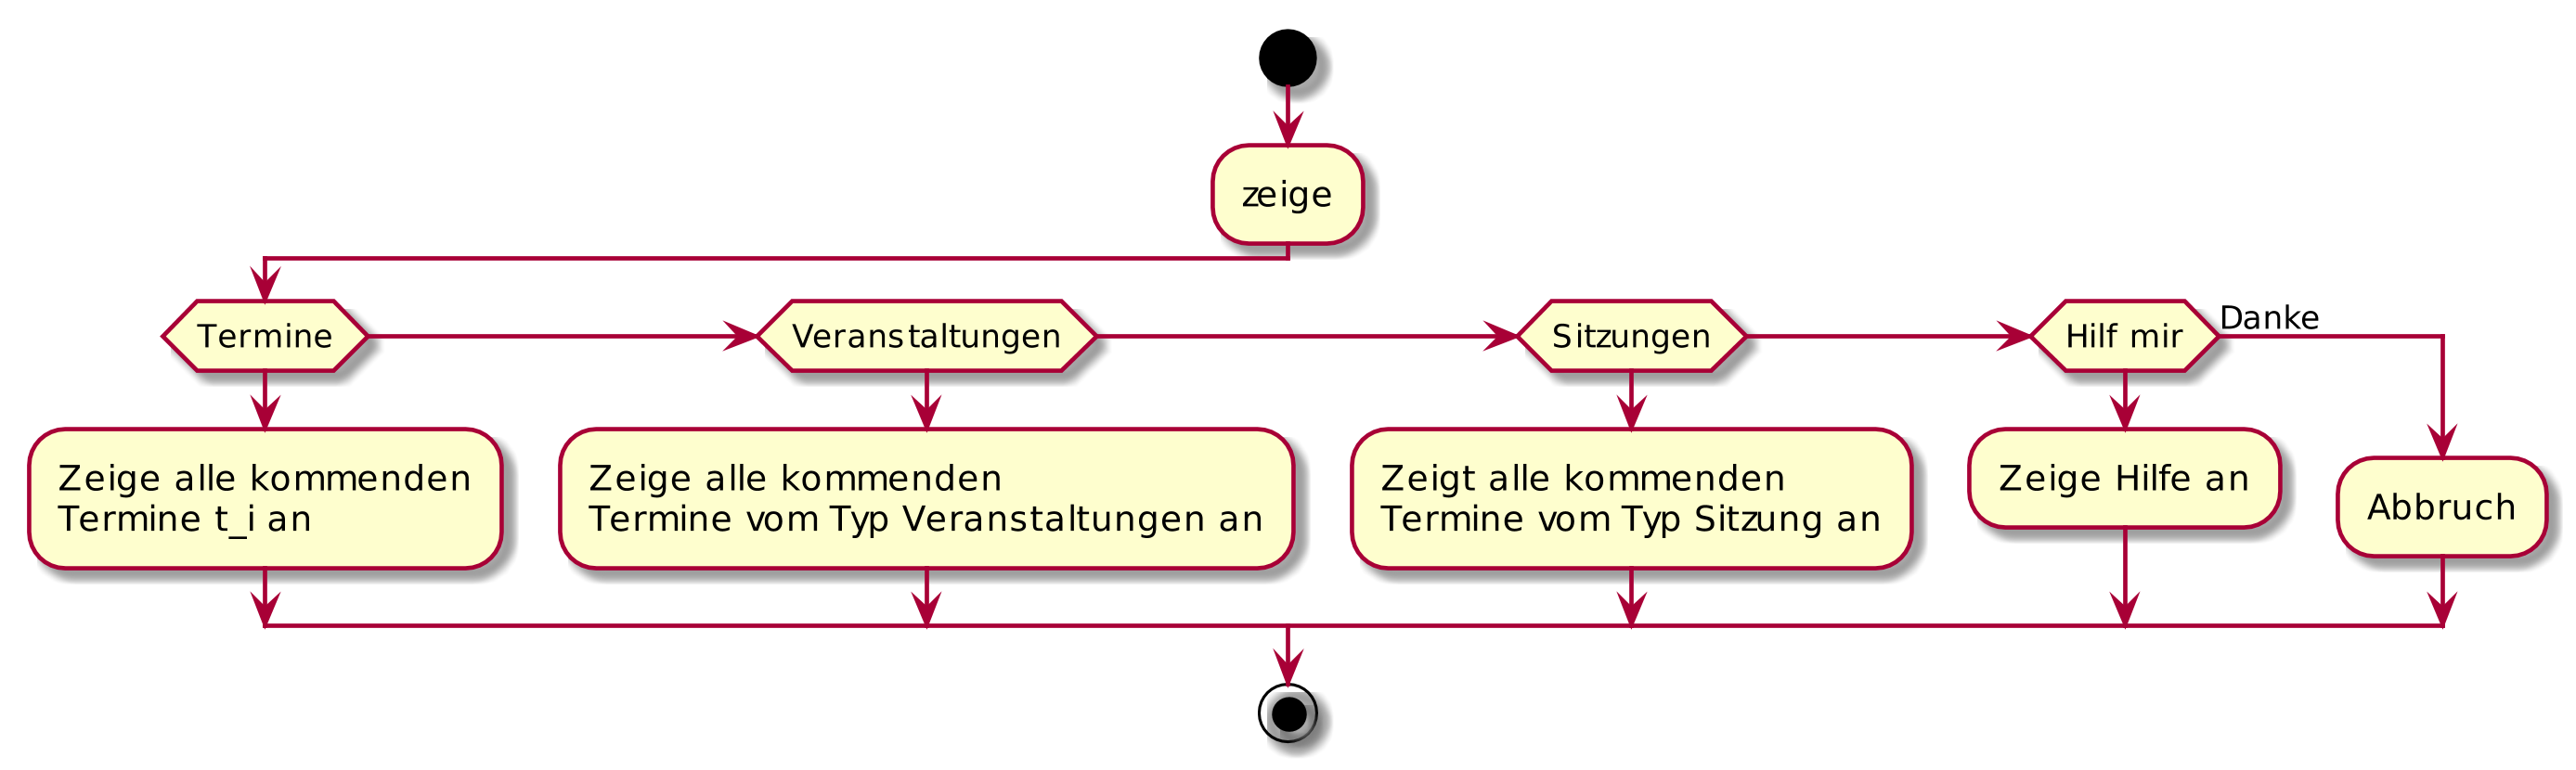
\includegraphics[width=0.9\textwidth]{../docs/uml/activity-zeige2.png}
    \caption{Aktivitätsdiagramme zum Anzeigen von Terminen}
    \label{img:activity-zeige}
\end{figure}

\begin{figure}[htbp]
    \centering
    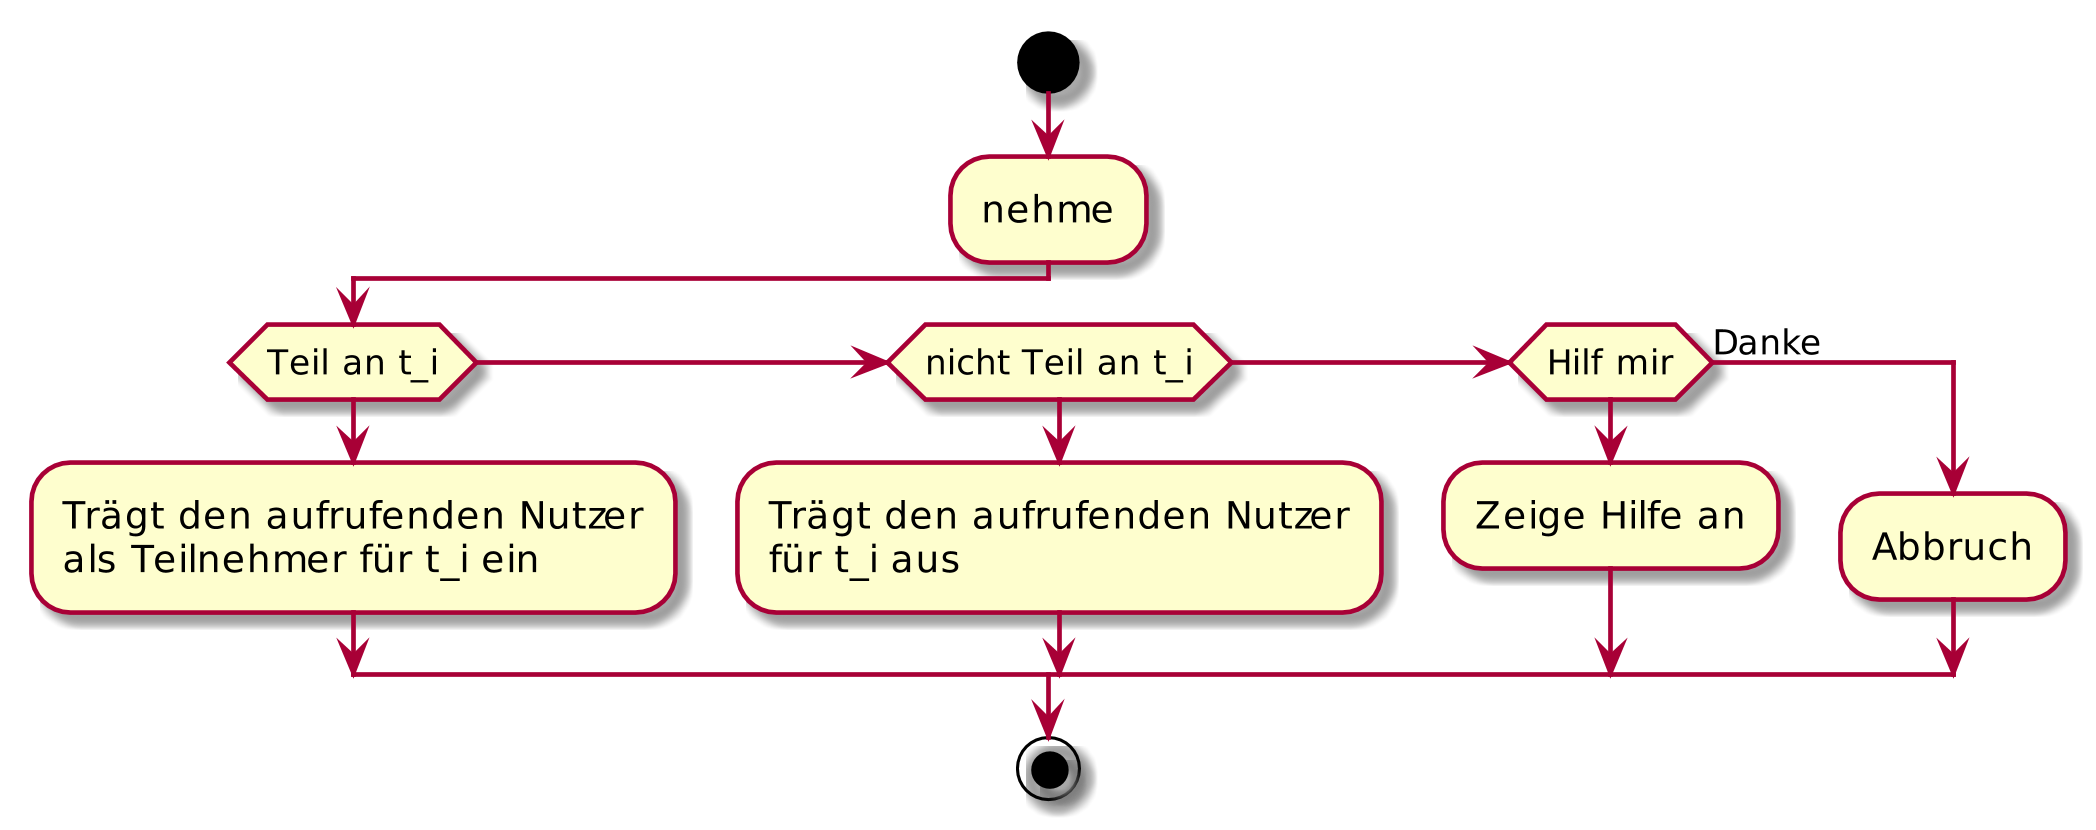
\includegraphics[width=0.7\textwidth]{../docs/uml/activity-teilnahme.png}
    \caption{Aktivitätsdiagramm zur Teilnahme an Terminen}
    \label{img:activity-teilnahme}
\end{figure}


\subsection{Datenbankschema}

Das Datenbankschema soll laut Anforderung unabhängig von einem spezifischen Chatbot nutzbar sein. Falls ein Chatbot ausgetauscht oder andere Interaktionsmethoden hinzugefügt werden, darf die Datenbank entsprechend keine Abhängigkeiten besitzen. Es wird deshalb ein Datenbankschema angelegt, welches nur die Terminverwaltung abbildet und anschließend eine Erweiterung hinzugefügt, welche die notwendigen Schlüssel auf die verwendete Plattform abbildet.

% Hier das DB-Schmea rein und eine Fremdschlüsseltabelle für die Slack-Nutzernamen und bla

\begin{figure}[htbp]
    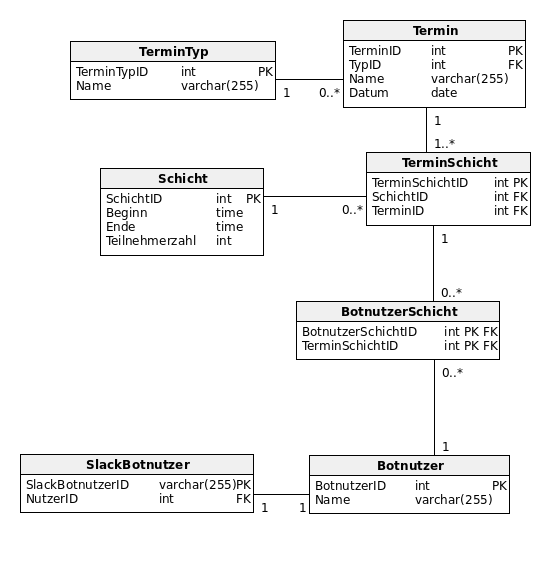
\includegraphics[width=\textwidth]{../docs/uml/Steckerbot-DB.png}
    \caption{Schema für die Termin-DB}
    \label{img:db-schema}
\end{figure}


\subsection{Kommunikationsschnittstellen}

Die kommunikation zwischen der Datenbank und dem Chatbot erfolgt auf dem gleichen Host, weshalb keine besonderen Fälle beachtet werden müssen. Der Kommunikationspfad zwischen dem Chatbot und Slack wird jedoch über ein Hochschulnetzwerk durchgeführt. In diesem sind in das Netzwerk des Clubs nur die Ports 80 und 443 freigegeben. Ausgehend ????????????????? doppeltes NAT aber Webseiten ok

Aus diesem Grund muss der Chatbot sich als Client mit Slack verbinden und darf keine Serveranwendung sein, welche ein Polling implementiert.

% vllt Grafik einfügen?


TODO: ERWEITERN
Slack hat eine option globale UIDs zum bot durchzuleiten. nützlich, wenn mehrere Workspaces genutzt werden - ist das der fall? ferdi fragen.

% Kommunikationspfade, Blockdiagramme, UML
% Datenhaltung, Datentransport, Sicherheit, Zukunftssicherheit, Austauschbarkeit, Robustheit, Erweiterbarkeit

\clearpage
\section{Realisierung des Modells}
\subsection{Datenbank}

Als Datenbank wurde aus den in \autoref{datenbankauswahl} genannten Gründen MySQL ausgewählt.
Für die Erstellung der Datenbank entschieden sich die Autoren für die Verwendung eines Hilfswerkzeugs, in dem das Modell abgebildet und eine Befehlskette ausgegeben wird. Dadurch sollte eine Abweichung der Realisierung vom Modell vermieden und eine rasche prototypische Verifizierung ermöglicht werden. Aktuell (März 2018) existiert kein anerkannter Standard (wie z.B. UML) zur Beschreibung von Datenbanken, weshalb sich die Autoren für das Hilfswerkzeug \enquote{Vertabelo} entschieden. Dieses gibt die notwendigen SQL-Befehle aus, welche direkt für die Erstellung der Datenbank verwendet werden können. Weiterhin können die unter \url{vertabelo.com} angelegten Datenbankmodelle von mehreren Nutzern verwendet werden, was insbesondere für die geplante Weiterverwendung der Datenbank nützlich sein kann.
Die bereits in \autoref{img:db-schema} gezeigte Datenbank ist unter \cite{VertabeloDesignYourDatabase2018} abrufbar. Der daraus generierte SQL-Code befindet sich im Anhang.


\subsection{Containerisierung}

Um das optionale Ziel der Containerisierung zu erreichen, wurde auf einen Standardcontainer der MySQL-Entwickler über Docker zurückgegriffen. Der Container zum Betrieb des Hubots basiert auf einem Alpine Linux-Container mit NodeJS, welcher mittels eines selbst entworfenen Dockerfiles erstellt wurde, welches in \autoref{lst:dockerfile} zu sehen ist.

% Die Autoren entschieden sich gegen den Bau eines eigenen Containers, um die Fehleranfälligkeit zu verringern und dokumentations- und supportkompatibel zu bleiben.

Docker ist eine Technologie zum Betrieb von Anwendungen in Containern, wobei jeder Container eine von den restlichen Containern isolierte Umgebung (Dateien, \linebreak Abhängigkeiten) erhält, dabei jedoch die Hardwareressourcen des Hostsystems mit anderen Containern teilt. Da diese Lösung wesentlich weniger Overhead bezüglich Speicher, Speicherplatz und Geschwindigkeit als eine Virtuelle Maschine bietet, eignen sich Container für die künstliche Abgrenzung vom Gesamtsystem und dadurch als einfach in den Produktiveinsatz zu überführende Lösung.

\subsubsection{Vergleich von Containerisierungslösungen}
Neben dem Einsatz der Containerlösung Docker wurden zu Projektbeginn Alternativen entsprechend \autoref{tab:docker-alternatives} betrachtet.

\begin{table}[H]
    \centering
    \begin{tabularx}{\textwidth}{|l|X|X|X|X|}
        \hline
        & \textbf{Docker} & \textbf{nativ} & \textbf{VirtualBox} & \textbf{Cloud} \\
        \hline
        Beschreibung & Umgebung für Linux-Container & lokale Installation der Anwendungen & Vollvirtuali- sierung inkl. Hardware & entfernte, dynamisch einsetzbare Ressourcen \\
        \hline
        Beispiel & docker pull mysql & apt install mysql & bitnami NodeJS VM & \url{heroku.com} \\
        \hline
        Geschwindigkeit     & $++$      & $+++$     & $+$   & $++++$ \\
        \hline
        Datensparsamkeit    & $++++$    & $++$      & $+++$ & $+$ \\
        \hline
        Portierbarkeit      & $++++$    & $+$       & $+++$ & $++$ \\
        \hline
        Persistenz          & $+$       & $+++$     & $++$  & $++++$ \\
        \hline
        \hline
        $\Sigma$            & 11        & 10        & 9     & 11 \\ 
        \hline
        \textbf{Ausschlusskriterium} & - & Testumgebung inhomogen, Serverinfrastruktur unbekannt & instabiles CLI (command line interface) & Datenschutz nicht gewährleistet, vendor-lock-in, laufende Kosten \\
        \hline
    \end{tabularx}
    \caption{Docker-Alternativen im Vergleich}
    \label{tab:docker-alternatives}
\end{table}

Der Vergleich der Docker-Alternativen erfolgte anhand einer positiven Gewichtung (Anzahl $+$) auf einer Skala von 1 bis 4. Dies ist für den groben Überblick ausreichend, bildet dabei aber keine detailliertere Gewichtung der Aspekte ab. Zur Abschätzung der Vor- und Nachteile reicht dieser grobe Vergleich jedoch aus. Die Gewichtung der Aspekte untereinander ist außerdem inhomogen. So ist die Anforderung der Datensparsamkeit z.B. wichtiger als die Geschwindigkeit. Daher sind die im folgenden näher erläuterten Punkte gesondert zu betrachten, da die Betrachtung der Summe über die Teilaspekte zum einen wenig aussagekräftig ist und zum anderen keine Form der Gewichtung der Vergleichskriterien beinhaltet.

\begin{itemize}
    \item Beispiel - ein charakteristischer Befehl/Referenz, siehe \cite{HubotDeploying2018}
    \item Geschwindigkeit - relative Zeit zur Ausführung der Anwendung
    \item Datensparsamkeit - Menge der ausgehenden Daten (weniger ist besser)
    \item Portierbarkeit - Grad der einfachen Portierung auf andere Systeme/Plattformen
    \item Persistenz - Möglichkeiten zur dauerhaften Datenspeicherung
\end{itemize}

Neben den positiven Kriterien, die sich untereinander nur qualitativ unterscheiden lassen, bestehen auch Ausschlusskriterien. Diese wurden hinsichtlich des Docker-Einsatzes \enquote{optimiert} und sind daher in anderen Kontexten kritisch zu betrachten. Die in diesem Projekt zu erfüllenden Aufgaben werden aber durch den Einsatz Dockers zu 100\% erfüllt.

\subsubsection{Entwicklungsumgebung mit Docker}

Basierend auf \autoref{img:deployment} ist die Systemumgebung für den Betrieb von Hubot mindestens aus den Komponenten \enquote{Chatbot} und \enquote{Termindatenbank} aufgebaut. Aus Gründen der Wartbarkeit, des fehlerminimierenden Betriebs und der offiziellen Empfehlung der Entwickler wird diese Trennung auch von den Docker-Containern aufrechterhalten.

Besondere Beachtung erfordert dabei die Verwaltung persistenter Daten, insbesondere der Datenbank. Da Docker-Container Daten standardmäßig nur flüchtig speichern, % Idempotenz kann man hier nicht wirklich sagen, da man die referenz auf einen container entfernen muss, bevor man ihn wieder starten kann, das ist gecheatet. finde ich dementsprechend gewagt
wird für den Erhalt der Datenbank ein persistentes Docker-Volume benötigt. Dafür wird ein \enquote{Volume} zwischen Hostsystem und Docker-Container eingebunden, so dass die Datenbank auch nach Beenden des Containers zur Verfügung steht.

Hinzu kommt ein weiterer Container zum Betrieb des eigentlichen Chatbots mittels NodeJS. Dieser wird mit dem gleichen virtuellen Netzwerk wie der DB-Container verbunden um Zugriff auf die Datenbank zu erhalten.

Weitere Einstellungen wie z.B. die zu öffnenden Ports folgen dem Paradigma \enquote{Convention over Configuration} (siehe \cite{NicholasChenConventionConfiguration2006}). Die Verbindung der Container untereinander erfolgt mittels docker-compose, in der docker-compose-Datei sind ebenfalls vordefinierte Standardwerte enthalten, welche schnell zum produktiven Einsatz führen (\cite{DockerCompose2018} und \autoref{lst:docker-compose}).
Dynamische Konfigurationen wie z.B. die UserID des Slackbots werden über entsprechende Umgebunsgvariablen in einer \verb+.env+-Datei übergeben und können problemlos während der Laufzeit geändert werden.

% \todo{docker-compose in den Anhang}
% docker-compose beschreiben


%hubot-docker bla


\subsection{Slackidentifizierung}

Die Identifizierung von Nutzern durch den Bot geschieht über die von Slack vergebene eindeutige Nutzeridentifizierungsnummer, welche über ein Nachrichtenobjekt innerhalb des Bots ausgelesen werden kann. Diese eindeutige Identifizierungsnummer wird durch den aufrufenden Nutzer in Slack in die Datenbank eingetragen, indem der Nutzer folgenden den Befehl aufruft: 
\texttt{@bob füge mich der Datenbank hinzu als <Vorname Nachname>}.

Der angegebene Name wird anschließend in der Nutzertabelle identifiziert und mit der SlackID verknüpft. Die Zuweisung kann nicht automatisch durch den in Slack angegebenen Namen geschehen, da dieser nicht gleich dem in der Datenbank als echten Namen eingetragenen Namen sein muss.


% anflanschung der slacknutzer-tabelle // vielleicht in eine separate db??? oder reicht ne tabelle / viele tabellen für viele plattformen aus

\subsection{Botrealisierung}
\subsubsection{Botname}
Da der Bot einen im deutschsprachigen Raum selten vorkommenden und zugleich kurzen und dadurch schnell zu schreibenden und leicht zu merkenden Namen erhalten sollte, entschieden sich die Autoren für den Namen Bob. Hierbei ist es nicht notwendig auf die Groß- und Kleinschreibung zu achten. Weiterhin wird der Bot im dynamischen Dropdownmenü innerhalb von Slack als Vorschlag angeboten, wenn dieser dem Raum hinzugefügt und direkt mittels einem \texttt{@}-Symbol adressiert wird. Die Autoren erhoffen sich dadurch eine einfachere Verwendung des Bots innerhalb der mobilen Applikation, da bei diesen die Schreibgeschwindigkeit geringer ist. Weiterhin kann dadurch eine größere Akzeptanz erreicht werden.

\subsubsection{Ereignisgesteuerte Aktionen}

Ereignisgesteuerte Aktionen werden nur ausgeführt, wenn ein Nutzer ein Ereignis auslöst. Der Bot interpretiert hierbei jede in den Chat geschriebene Nachricht und prüft diese auf ein Muster mithilfe eines regulären Ausdrucks. Da die Definitionen der ereignisgesteuerten Aktionen in der EBNF geschrieben wurden, können diese ohne umfangreiche Konvertierung mit einem regulären Ausdruck implementiert werden. Hierbei ist die Groß- und Kleinschreibung und die Anzahl an Leerzeichen zwischen den Schlagwörtern unwichtig.

\subsubsection{Zeitgesteuerte Aktionen}

Die zeitgesteuerten Aktionen beschränken sich auf die selbstständige Erinnerung an Termine durch den Bot. Der Bot darf in dieser Hinsicht keinen Zwischenspeicher besitzen, da neue Termine nicht durch den Bot eingetragen werden müssen und von einer externen Anwendung kommen können. Der gemeinsame Zugriffspunkt ist die Datenbank. Aus diesem Grund fragt der Bot die Datenbank periodisch ab.

Die Autoren legten eine zeitlich positive Abweichung von 5 Minuten als akzeptablen Wert bezüglich des echten Termins fest. Dieser entstand durch die Überlegung, wie groß die maximale Dauer für eine Abfrage an die Datenbank sein kann. Bei einer Teilnehmeranzahl von im $\o$ 10, einer Mitgliedsdauer von 50 Jahren und einer implementierungstechnisch pessimistisch angenommenen wöchentlichen Teilnahme an einer Veranstaltung pro Mitglied würden $52 \cdot 50 \cdot 10$ Terminschichteinträge vorhanden sein. Da eine Abfrage des nächsten Termins auf einem aktuellen Laptop $\approx 60\mu s$ dauert, ist eine obere Grenze von $52 \cdot 10 \cdot 50 \cdot 60 \mu s=1,56s=\varepsilon $ zu erwarten.

Der Bot fragt die Datenbank periodisch aller 3 Minuten auf nächstgelegene Termine ab, während die zu betrachtenden Termine in einer Zeitspanne von 5 Minuten liegen. Da der Bot eine maximale Abfragezeit von $\varepsilon + 3min$ hat, liegt der Abtastzeitpunkt immer innerhalb der 5 Minuten-Spanne. Nachfolgende Grafik verdeutlicht dies.

%Anhang mit botcode dranheften

%wie erweiterbarkeit realisiert? - include module bla, file x

% Warum welche Sprache
% Warum Abkürzungen im ggs zu Modell genommen
% Welche praktischen Hürden überwunden

\clearpage
\section{Analyse}
% Alle Anforderungen erfüllt?
% Wie gemessen?
% Blockdiagramme, MSCs, Fehlerbetrachtung
% Performance - Latenz?

\clearpage
\section{Fazit}
% Funzt? Jo
% Was wurde erledigt, was ¬ und warum?

\clearpage
\section{Aussicht}
% Empfehlungen für Verbesserungen, Erweiterungsmöglichkeiten, ...

\clearpage
\section{Benutzung des Endprodukts}
% Wo Daten eingeben, Wie per Hand testen, Wie Komponenten verbinden, (minimal) Beispiel


%Literatur
\nocite{GitHubGettingStartedHubot}
\nocite{BotkitBotkitToolkitbuilding}
\nocite{SlackConversationsAPI}
